\documentclass[12pt, a4paper]{article}

\usepackage[utf8]{inputenc}
% Limit the page margin to only 1 inch.
\usepackage[margin=1in]{geometry}

%Imports biblatex package
\usepackage[
backend=biber,
style=alphabetic
]{biblatex}
%\addbibresource{../../mth342.bib}

% Enables the `align' environment.
\usepackage{amsmath}
% Provides useful environments, such as:
% - \begin{proof} ...\end{proof}
\usepackage{amsthm}
\usepackage[most]{tcolorbox}

\newtheorem*{proposition}{Proposition}
\theoremstyle{definition}
\newtheorem*{definition}{Definition}

% Enables using \mathbb{}, for example \mathbb{N} for the set of natural numbers.
\usepackage{amssymb}

% Allows using letters in enumerate list environment. Use, for example:
%\begin{enumerate}[label=(\alph*)]
% ...
%\end{enumerate}
\usepackage[inline]{enumitem}

% Enable importing external graphic files and provides useful commands, like \graphicspath{}
\usepackage{graphicx}
% Images are located in a directory called "images" in the current directory.
\graphicspath{{./images/}}

% Make links look better by default.
% See: https://tex.stackexchange.com/questions/823/remove-ugly-borders-around-clickable-cross-references-and-hyperlinks
\usepackage[hidelinks]{hyperref}
\usepackage{xcolor}
\hypersetup{
	colorlinks,
	linkcolor={red!50!black},
	citecolor={blue!50!black},
	urlcolor={blue!80!black}
}

% Code Listings. Source:
% https://stackoverflow.com/questions/3175105/inserting-code-in-this-latex-document-with-indentation
\usepackage{listings}
\usepackage{color}

\definecolor{dkgreen}{rgb}{0,0.6,0}
\definecolor{gray}{rgb}{0.5,0.5,0.5}
\definecolor{mauve}{rgb}{0.58,0,0.82}

\lstset{frame=tb,
	language=Java,
	aboveskip=3mm,
	belowskip=3mm,
	showstringspaces=false,
	columns=flexible,
	basicstyle={\small\ttfamily},
	numbers=none,
	numberstyle=\tiny\color{gray},
	keywordstyle=\color{blue},
	commentstyle=\color{dkgreen},
	stringstyle=\color{mauve},
	breaklines=true,
	breakatwhitespace=true,
	tabsize=3
}

\newcommand{\prob}{\text{P}}
%\newcommand{\complement}{\mathsf{c}}

\title{Lecture 05: MATH 342W: Introduction to Data Science and Machine Learning}
\author{Sergio E. Garcia Tapia\thanks{Based on lectures of Dr. Adam Kapelner at Queens College.
		See also the \href{https://github.com/kapelner/QC_MATH_342W_Spring_2025}{course GitHub page}.}}
\date{February 11, 2025 (last updated \today)}

\begin{document}
	\maketitle
	
	\subsection*{Recap of Perceptron}
	Suppose $\mathcal{X}$ is a $p$-dimensional feature space and $\mathcal{Y}$ is a
	binary response space. Let $\mathbb{D}$ be a data set of points $(\mathbf{x}_i, y_i)$,
	where $\mathbf{x}_i\in \mathcal{X}$, $y_i\in \mathcal{Y}$, and $i$ is an integer
	satisfying $1\leq i\leq n$. We saw that if $\mathbb{D}$ is perfectly linearly
	separable, then the Perceptron Learning Algorithm is guaranteed to converge,
	and it produces a feature weight vector $\mathbf{w}\in\mathbb{R}^p$ and a bias
	$b\in\mathbb{R}$ defining a hyperplane that perfectly separates the data.
	Put another way, the indicator function $\mathbb{I}_{\mathbf{w}\cdot \mathbf{x}+b\geq 0}$
	has zero misclassification error.
	There are infinitely-many such hyperplanes, and a natural question is: \emph{is there a best one}?
	
	\subsection*{The Support Vector Machine (SVM)}
	Suppose $\mathbb{D}$ is perfectly linearly separable and that we have obtained a hyperplane
	that separates the data set.
	Define the \textbf{margin} as the distance from a hyperplane that separates the data to the closest point
	in either side of the hyperplane. In this section, we seek algorithm to determine
	the \textbf{maximum margin hyperplane}, which was proven in 1998 to be the optimal
	binary classifier for linearly separable data.
	
	\begin{figure}[h]
		\centering
		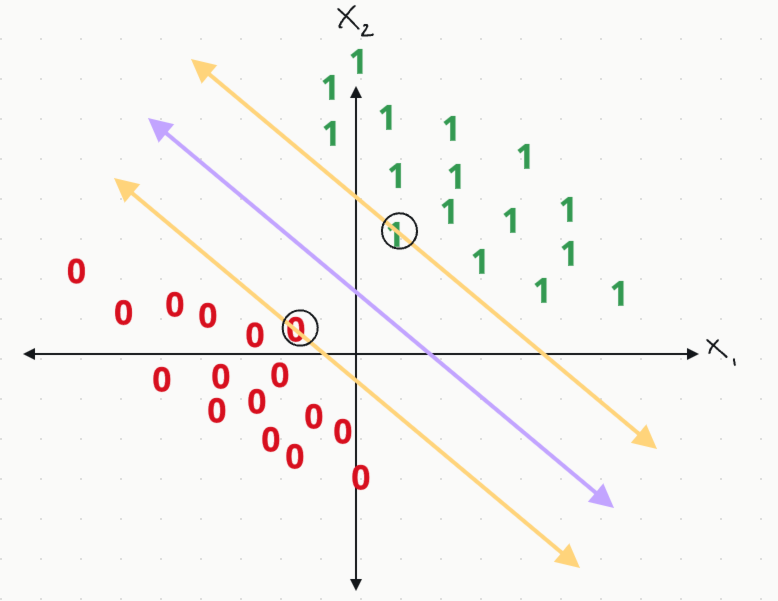
\includegraphics[width=0.6\textwidth]{max-margin-hyperplane}
		\caption{A perfectly linearly separable data set $\mathbb{D}$ separated by
		a maximum margin hyperplane colored purpled. The points corresponding to the circled responses
		are the support vectors of this hyperplane.}
		\label{fig:max-margin-hyperplane}
	\end{figure}
	See Figure~\ref{fig:max-margin-hyperplane}.
	The classifier model is called the \textbf{support vector machine (SVM)}. In this context,
	the points $\mathbf{x}_i$ that determine this margin are referred to as the \textbf{support vectors}.
	
	As a first step towards deriving this algorithm, let's re-write the hypothesis set
	as follows:
	\begin{align*}
		\mathcal{H} = \{\mathbb{I}_{\mathbf{w}\cdot \mathbf{x}-b\geq 0}: \mathbf{w}\in\mathbb{R}^p, b\in\mathbb{R}\}
	\end{align*}
	A plane specified by the equation $\mathbf{w}\cdot \mathbf{x}-b=0$ is said to be in
	\emph{Hesse Normal Form}. For example, suppose we are in $\mathbb{R}^2$, and we have the
	equation of a line $x_2=2x_1+3$. Then we can re-write it as $2x_1-x_2+3=0$, or in vector notation:
	\begin{align*}
		\underbrace{
		\begin{bmatrix}
			2\\
			-1
		\end{bmatrix}
		}_{\mathbf{w}}
		\cdot
		\underbrace{
		\begin{bmatrix}
			x_1\\
			x_2
		\end{bmatrix}
		}_{\mathbf{x}}
		-
		\underbrace{(-3)}_{b}=0
	\end{align*}
	Thus, a hyperplane in $\mathbb{R}^2$ is a line, while a hyperplane in $\mathbb{R}^3$ is
	a 2-dimensional plane, and a hyperplane in $\mathbb{R}^p$ is a $(p- 1)$-dimensional space
	that generalizes this notion.
	
	Note that since $\mathbf{w}\cdot \mathbf{x}-b=0$, then for any $c\neq 0$, we have
	\begin{align*}
		c(\mathbf{w}\cdot \mathbf{x}-b)=c(0)=0.
	\end{align*}
	Hence, the Hesse normal form is ``overdetermined", in the sense that there are infinitely many
	ways to express this hyperplane. Let $\ell$ refer to the hyperplane defined by the equation
	$\mathbf{w}\cdot \mathbf{x}-b=0$. If $\delta>0$, we can define $\ell_L$ to
	be hyperplane parallel to $\ell$ obtained by shifting $\ell$ by $-\delta$ (down)
	and $\ell_U$ be obtained by shifting $\ell$ by $+\delta$ (up).
	\begin{figure}
		\centering
		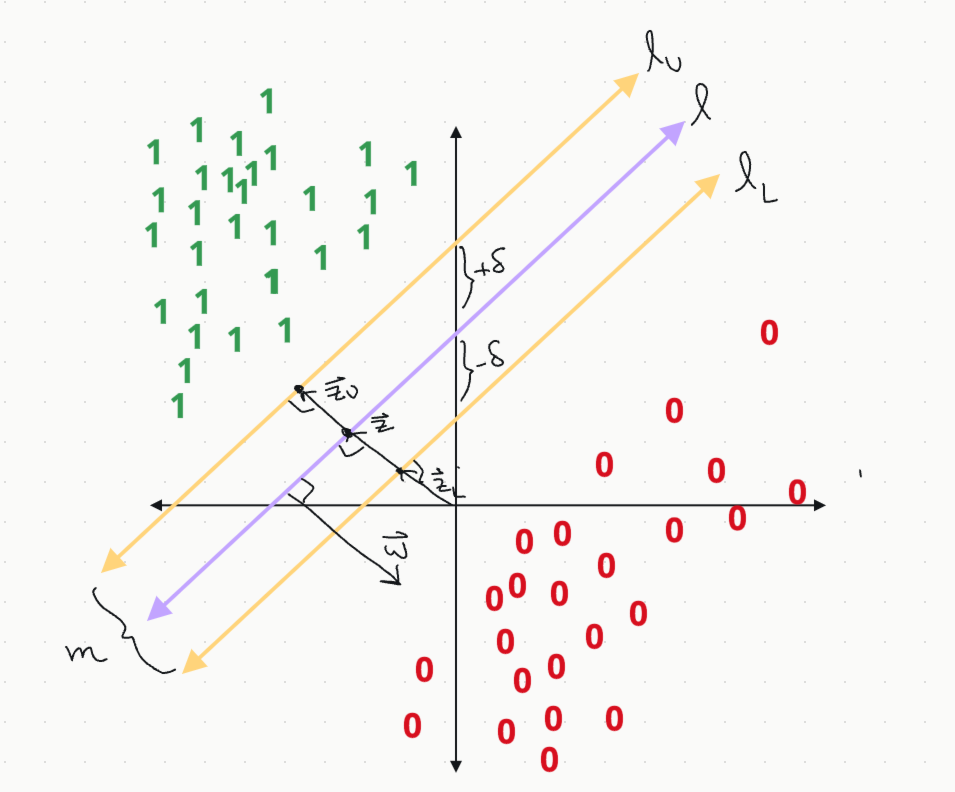
\includegraphics[width=0.7\textwidth]{svm-derivation-z-vectors}
		\caption{$\ell$ perfectly separates data set $\mathbb{D}$. Here $\ell_U$ and
		$\ell_L$ are obtained by shifting $\ell$ by $\delta$. $\mathbf{w}$ is normal to $\ell$.}
		\label{fig:svm-derivation}
	\end{figure}
	See Figure~\ref{fig:svm-derivation}.
	
	Define $m>0$ to be the perpendicular distance between $\ell_L$ and $\ell_U$.
	In Hesse Normal form, $\mathbf{w}$ is perpendicular to $\ell$, and it is called the
	\textbf{normal vector}. Next, we define the following vectors:
	\begin{itemize}
		\item Let $\mathbf{w}_0:=\frac{\mathbf{w}}{\|\mathbf{w}\|}$ be the unit vector in the direction
		of $\mathbf{w}$.
		\item Let $\mathbf{z}$ be a normal vector residing on $\ell$.
		\item Let $\mathbf{z}_L$ be a normal vector residing on $\ell_L$.
		\item Let $\mathbf{z}_U$ be a normal vector residing on $\ell_U$.
	\end{itemize}
	Since $\mathbf{z}$ is normal to $\ell$, it must be in $\text{span}(\mathbf{w})$,
	so $\exists_{\alpha\in\mathbb{R}}$ such that $\alpha\neq0$ and $\mathbf{z}=\alpha \mathbf{w}_0$.
	On the other hand, $\mathbf{z}\in \ell$, so it must satisfy the hyperplane equation
	for $\ell$, i.e., $\mathbf{w}\cdot \mathbf{z}-b=0$. Combining the two, we get
	\begin{align*}
		\mathbf{w}\cdot \mathbf{z}-b&=0\\
		\mathbf{w}\cdot (\alpha \mathbf{w}_0)-b&=0\\
		\mathbf{w}\cdot \left(\alpha\cdot \frac{\mathbf{w}}{\|\mathbf{w}\|}\right)-b&=0\\
		\alpha \frac{\|\mathbf{w}\|^2}{\|\mathbf{w}\|}-b&=0\\
		\alpha &= \frac{b}{\|\mathbf{w}\|}
	\end{align*}
	Recalling $\mathbf{z}=\alpha \mathbf{w}_0$, we can write
	\begin{align*}
		\mathbf{z}=\frac{b}{\|\mathbf{w}\|}\mathbf{w}_0
	\end{align*}
	A similar derivation shows that $\mathbf{z}_U=\alpha_U\mathbf{w}_0$ (replacing
	$b$ with $b+\delta$) yields
	\begin{align*}
		\mathbf{w}\cdot \mathbf{z}_U-(b+\delta)&=0\\
		\mathbf{z}_U=\frac{b+\delta}{\|\mathbf{w}\|}\mathbf{w}_0
	\end{align*}
	And analogously for $\ell_L$ (replacing $b$ with $b-\delta$), we have
	\begin{align*}
		\mathbf{z}_L =\frac{b-\delta}{\|\mathbf{w}\|}\mathbf{w}_0
	\end{align*}
	Recall we defined $m$ as the perpendicular distance between $\ell_L$ and $\ell_U$.
	We want $m$ to be maximized to find the maximum margin hyperplane. From our
	calculations and the diagram in Figure~\ref{fig:svm-derivation}, we see that
	\begin{align*}
		m &= \|\mathbf{z}_U-\mathbf{z}_L\|\\
		&=\left\|
		\frac{b+\delta}{\|\mathbf{w}\|}\mathbf{w}_0-\frac{b-\delta}{\|\mathbf{w}\|}\mathbf{w}_0
		\right\|\\
		&=\left\|\frac{2\delta}{\|\mathbf{w}\|}\mathbf{w}_0\right\|\\
		&=\frac{2\delta}{\|\mathbf{w}\|}
	\end{align*}
	since $\mathbf{w}_0$ is a unit vector. Therefore, to maximize $m$, we need to minimize
	$\|\mathbf{w}\|$. However, we need a condition for minimization. We'll derive this next.
	
	Recall that the Hesse normal form for $\ell$ is overdetermined, so we can pick any $c\neq 0$
	and we will have $c(\mathbf{w}\cdot \mathbf{x}-b)=0$. Pick $c=\frac{1}{\delta}$,
	thereby constraining us to one solution. Then there is one $\mathbf{w}$ and one $b$
	that specify any hyperplane. Using the equation for $\ell_U$, we will write
	\begin{align*}
		\mathbf{w}\cdot \mathbf{x}-(b+\delta)&=0\\
		\frac{1}{\delta}\mathbf{w}\cdot \mathbf{x}-\frac{1}{\delta}(b+\delta)&=0\\
		\underbrace{\frac{\mathbf{w}}{\delta}}_{\mathbf{w}'}\cdot \mathbf{x}
		-\left(\underbrace{\frac{b}{\delta}}_{b'}-1\right)&=0\\
		\mathbf{w}'\cdot \mathbf{x}-(b'+1)&=0,\quad i \text{ such that } y_i=1
	\end{align*}
	Likewise, for $\ell_L$, we have $\mathbf{w}'\cdot \mathbf{x}-(b'-1)=0$. Now,
	on and above $\ell_U$, we know that all $y_i=1$ (recall the candidate functions are indicator
	functions), and hence for such $i$ we have
	\begin{align*}
		\mathbf{w}'\cdot \mathbf{x}_i-(b'+1)&\geq 0\\
		\mathbf{w}'\cdot \mathbf{x}_i-b'&\geq 1\\
		\frac{1}{2}\left(\mathbf{w}'\cdot \mathbf{x}_i-b'\right)&\geq \frac{1}{2}\\
		\left(y_i-\frac{1}{2}\right)\left(\mathbf{w}'\cdot \mathbf{x}_i-b'\right)&\geq \frac{1}{2},
		\quad i \text{ such that }y_i=1
	\end{align*}
	where we replaced $\frac{1}{2}$ with $y_i-\frac{1}{2}$ since $y_i=1$. Similarly,
	for all $i$ such that $y_i=0$, we are below $\ell_L$, and hence
	\begin{align*}
		\mathbf{w}'\cdot \mathbf{x}_i-(b'-1)&\leq 0\\
		\mathbf{w}'\cdot \mathbf{x}_i-b'&\leq -1\\
		-\frac{1}{2}\left(\mathbf{w}'\cdot \mathbf{x}_i-b'\right)&\geq \frac{1}{2}\\
		\left(y_i-\frac{1}{2}\right)\left(\mathbf{w}'\cdot \mathbf{x}_i-b'\right)&\geq \frac{1}{2},
		\quad i \text{ such that } y_i=0
	\end{align*}
	since $y_i=0$. Since the same inequality holds for all $i$, we can write
	\begin{align}
		\left(y_i-\frac{1}{2}\right)\left(\mathbf{w}'\cdot \mathbf{x}_i-b'\right)&\geq \frac{1}{2},\quad
		\text{ for all integers $i$ such that } 1\leq i\leq n
		\label{eqn:condition-svm}
	\end{align}
	Therefore Equation (\ref{eqn:condition-svm}) is our minimization condition.
	Assuming the data set is perfectly linearly separable, we have the following algorithm:
	\begin{align*}
		\mathcal{A}:\mathbf{w}^*, b^*=
		\underset{\substack{\mathbf{w}'\in\mathbb{R}^p \\b'\in\mathbb{R}}}{\text{argmin}}
		\{\|\mathbf{w}'\|\},\quad \forall_i:\text{Equation (\ref{eqn:condition-svm}) holds.}
	\end{align*}
	This is the \textbf{support vector machine}, and we use the candidate set
	\begin{align*}
		\mathcal{H}=\{\mathbb{I}_{\mathbf{w}\cdot\mathbf{x}-b\geq 0}:\mathbf{w}\in\mathbb{R}^p, b\in\mathbb{R}\}
	\end{align*}
	There is no closed form solution; you need to use an optimization algorithm to find
	$\mathbf{w}^*$ and $b^*$.
	
	If $\mathbb{D}$ is not linearly separable, then there is no maximum margin hyperplane,
	and we cannot use the SVM. However, we can tweak the algorithm to arrive at a similar algorithm
	that lets us do binary classifications.
	\begin{figure}
		\centering
		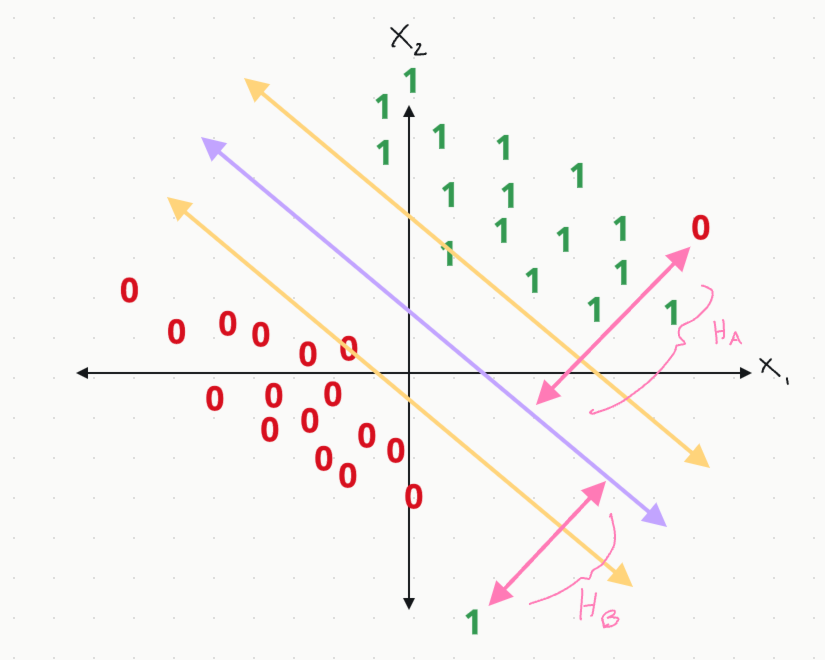
\includegraphics[width=0.7\textwidth]{non-linearly-separable-dataset}
		\caption{A data set that is not linearly separable.}
		\label{fig:non-linearly-separable-D}
	\end{figure}
	Consider the data set in Figure~\ref{fig:non-linearly-separable-D}, which is not
	perfectly linearly separable. For the two points in the diagram that are on the ``wrong side"
	(misclassified), let $i=A$ and $i=B$ be their corresponding indices. Then for these points,
	the condition of the indicator function is not satisfied, and hence we have
	\begin{align*}
		\left(y_A-\frac{1}{2}\right)(\mathbf{w}\cdot\mathbf{x}_A-b)&<\frac{1}{2}\\
		\left(y_B-\frac{1}{2}\right)(\mathbf{w}\cdot\mathbf{x}_B-b)&<\frac{1}{2}
	\end{align*}
	In fact, for all such $i$ that are misclassified, we can express this as an equation
	by choosing $d_i>0$ such that
	\begin{align}
		\left(y_i-\frac{1}{2}\right)(\mathbf{w}\cdot\mathbf{x}_i-b)&=\frac{1}{2}-d_i\nonumber\\
		d_i &= \frac{1}{2}-\left(y_i-\frac{1}{2}\right)(\mathbf{w}\cdot\mathbf{x}_i-b)\label{eqn:hinge_error}
	\end{align}
	We call $d_i$ the \textbf{severity of the error}. Now define $H_i$ by
	\begin{align*}
		H_i &:= \max \left\{
		0, d_i
		\right\}
	\end{align*}
	The $\max$ function assigns zero error to all observations that are correctly classified, and $d_i$
	where they are misclassified. This is called the \textbf{hinge error}.
	Ideally, we would want the hinge error to be zero, which would imply perfect linear separability.
	Let's define the \textbf{sum of hinge errors}:
	\begin{align}
		SHE := \sum_{i=1}^{n}\max\{0, d_i\},\label{eqn:SHE}
	\end{align}
	where $d_i$ is given by Equation~(\ref{eqn:hinge_error}).
	We want to minimize $SHE$. We have a wedge that separates most of the data, but we want
	to minimize the hinge errors simultaneously. That is, we want to minimize $SHE$
	while maximizing $m$ (as defined earlier), and the latter is equivalent to minimizing $\|\mathbf{w}\|$.
	This leads to the following algorithm (by Vaphik in 1963):
	\begin{align*}
		\mathcal{A}_{\lambda}:\mathbf{w}^*, b^*=
		\underset{\substack{\mathbf{w}'\in\mathbb{R}^p \\b'\in\mathbb{R}}}{\text{argmin}}
		\left\{\frac{1}{n}SHE+\lambda |\mathbf{w}'\|\right\}
		,\quad \forall_i:\text{Equation (\ref{eqn:condition-svm}) holds.}
	\end{align*}
	where $\frac{1}{n}SHE$ is the average $SHE$, and $SHE$ is given by Equation~(\ref{eqn:SHE}).
	Here, $\lambda>0$ and it is called a \textbf{hyperparameter}, meaning that the value of $\lambda$
	is a subjective choice that you are obligated to make. Each algorithm is indexed by
	$\lambda$, so we have an infinite family of algorithms. The question of course is how
	to choose a $\lambda$ that ensures our algorithm performs well.
	\pagebreak
%	\printbibliography
\end{document}